\subsection{CV-maximization for efficient visual feature extraction}
\label{sec:cv_algorithm}

We translate the framework's principle---CV as the macroscopic coordinate of efficient codes---into an artificial learning algorithm.  Natural-image patches are well-modeled as sparse mixtures of localized features whose coefficient distributions in over-complete dictionaries are heavy-tailed and approximately Gibbs-exponential \cite{13,field_relations_1987}; the patch-wise coefficient vector $\{|a_i|\}$ is therefore a natural analogue of the response distribution $p(r)$, and direct CV maximization should steer the dictionary toward a more efficient code without specifying a prior shape.  Classical sparse-coding models \cite{37} instead impose a fixed heavy-tailed prior (e.g., Cauchy \cite{38}); because the optimization jointly updates basis functions and coefficients through a non-convex procedure, the resulting activity distribution is not guaranteed to match the assumed prior, and the regularization strength offers no principled control over macroscopic coding statistics.

We replace the fixed prior with direct maximization of the population CV:
\begin{align}
L = \sum_{x,y} \Bigl[ I(x,y) - \sum_i a_i \phi_i(x,y) \Bigr]^2 - \alpha \cdot \mathrm{CV}(\mathbf{a}),
\end{align}
where $\mathrm{CV}(\mathbf{a})$ is computed over $\{|a_i|\}$ for each patch and the regularization weight $\alpha$ is gated by current reconstruction error so that the dictionary recovers Null-comparable RE before sparsity-promoting pressure is applied (Methods).  Coding efficiency is $\mathrm{ICE} = -\log_2(\mathrm{RE})/\bar{a}$ in bits per activation, where $-\log_2(\mathrm{RE})$ approximates the mutual information between input and reconstruction under a Gaussian additive-noise model (Methods).

Three sparse-coding models---unregularized Null, Cauchy-prior SparseNet, and CV-max---were trained on $16\times 16$ van Hateren patches.  CV-max recovers V1-like localized, oriented, bandpass receptive fields without hand-selected priors (Fig.~\ref{fig:CV-max}B).  In the pooled $|a|$ density (Fig.~\ref{fig:CV-max}C), Null tracks the $L_1$/Laplace exponential baseline; CV-max simultaneously raises the zero mass ($70.7\%$ vs.\ Null $65.7\%$) and extends the tail above Null---the heavier-tailed Gibbs solution expected under effectively sublinear cost (Supp.~Note ``Sublinear cost extension'').  SparseNet departs in the opposite direction (lowest zero mass $63.2\%$, faster-decaying tail), consistent with the Cauchy prior softening the L1 gradient near zero and over-suppressing large-amplitude features.  Reconstruction quality (SSIM, Fig.~\ref{fig:CV-max}D) and L2 reconstruction error (Supp.~Fig.~S5) place CV-max ($\mathrm{SSIM}=0.423$) close to Null ($0.444$) and well above SparseNet ($0.322$); CV-max reduces mean activation by $\sim 14\%$ relative to Null ($\bar a=0.050$ vs.\ $0.058$), while SparseNet reaches a lower $\bar a=0.042$ only at the cost of the largest RE.  CV-max also attains the highest pairwise basis-function independence (Fig.~\ref{fig:CV-max}E).  The combination yields the highest ICE (Fig.~\ref{fig:CV-max}F): $13.45$ bits/activation vs.\ Null $12.26$ and SparseNet $12.17$ ($\sim +1.2$ bits/activation; all pairwise $p<10^{-4}$).  A weight-sweep ablation across all three methods (Supp.~Fig.~S8 and Supp.~Note ``CV-max ablation'') confirms that the CV-max advantage holds at matched mean activation ($\Delta\mathrm{ICE}=+0.52$) and matched RE ($\Delta\mathrm{ICE}=+0.12$), and is not an artefact of one regularization weight.  Within this matched setup, targeting CV directly yields a more favourable efficiency--fidelity Pareto position than the Cauchy-prior baseline---a transferable design heuristic, not a claim of general superiority over sparse coding.

\begin{figure*}
\centering
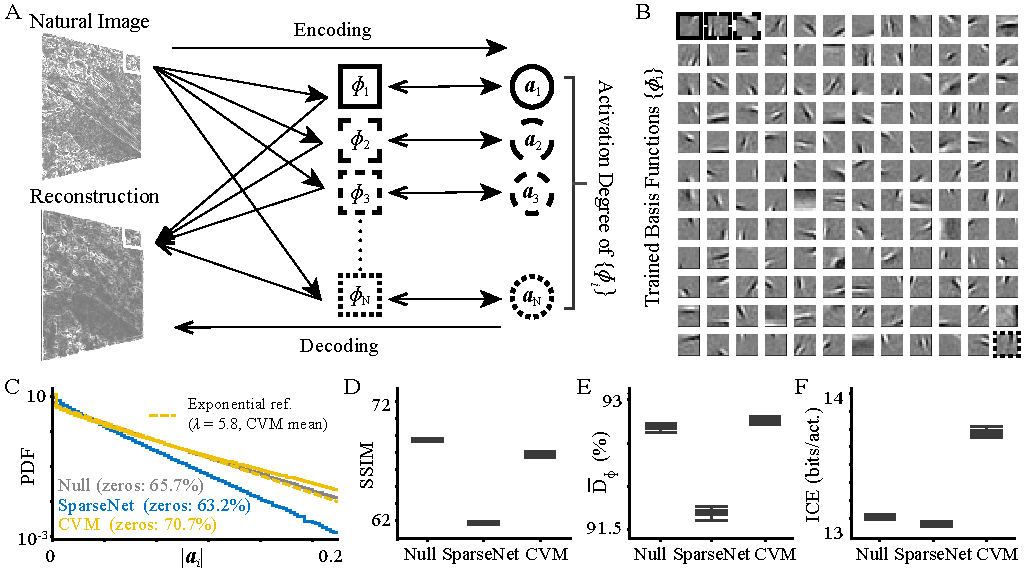
\includegraphics[scale=0.75]{figures/Figure6.pdf}
\caption{\textbf{CV-maximization yields higher cost-normalized efficiency than fixed-prior sparse coding.}
(\textbf{A})~Encoding/decoding schematic on $16\times 16$ natural-image patches; population CV of activation coefficients $\{a_i\}$ over basis functions $\{\phi_i\}$ is maximized with an RE-gated regularizer (Methods).
(\textbf{B})~Learned basis functions from CV-max: localized, oriented, bandpass.
(\textbf{C})~Pooled $|a|$ density (log-$y$, exact zeros excluded; zero-fractions in legend); dashed line: exponential reference ($\lambda=5.8$, CV-max mean).  Null (grey) tracks the L1/Laplace baseline; CV-max (yellow) has the highest zero mass ($70.7\%$) and lies above Null in the tail; SparseNet (blue) decays faster and has the lowest zero mass.
(\textbf{D})~SSIM: Null $0.444 \approx$ CVM $0.423 >$ SparseNet $0.322$.
(\textbf{E})~Pairwise basis independence $\bar{D}_\phi$: CVM $92.76\% >$ Null $92.68\% >$ SparseNet $91.70\%$.
(\textbf{F})~ICE ($-\log_2 \mathrm{RE}/\bar{a}$, bits/activation): CVM $13.45 >$ Null $12.26 >$ SparseNet $12.17$ ($\approx +1.2$ bits/activation).
All pairwise comparisons in D--F: $p<10^{-4}$.}
\label{fig:CV-max}
\end{figure*}
